\documentclass[border=6pt,tikz]{standalone}
\usepackage{tikz}
\usepackage{amsmath,amssymb}
\usetikzlibrary{arrows.meta,positioning,fit,backgrounds,calc,shapes.geometric,decorations.pathreplacing,patterns}
\definecolor{ink}{HTML}{1B2430}
\definecolor{muted}{HTML}{6B7785}
\definecolor{accent}{HTML}{2F6FB5}
\definecolor{accent2}{HTML}{C1611F}
\definecolor{good}{HTML}{2E7D5B}
\definecolor{soft}{HTML}{EDF2F7}
\definecolor{soft2}{HTML}{FBEDE2}
\definecolor{soft3}{HTML}{E6F0E9}
\tikzset{
  box/.style={draw=ink,line width=.7pt,rounded corners=2pt,fill=soft,inner sep=4pt,align=center,font=\sffamily\small},
  boxa/.style={box,fill=soft2},
  boxb/.style={box,fill=soft3},
  plain/.style={align=center,font=\sffamily\small,text=ink},
  tiny/.style={align=center,font=\sffamily\scriptsize,text=muted},
  ar/.style={-{Stealth[length=2.4mm]},draw=ink,line width=.7pt},
  arm/.style={-{Stealth[length=2.4mm]},draw=muted,line width=.6pt,dashed},
  nd/.style={circle,draw=ink,line width=.7pt,fill=white,minimum size=7mm,inner sep=0pt,font=\sffamily\scriptsize},
  ndf/.style={nd,fill=soft},
  ndt/.style={nd,fill=soft2},
}

\begin{document}
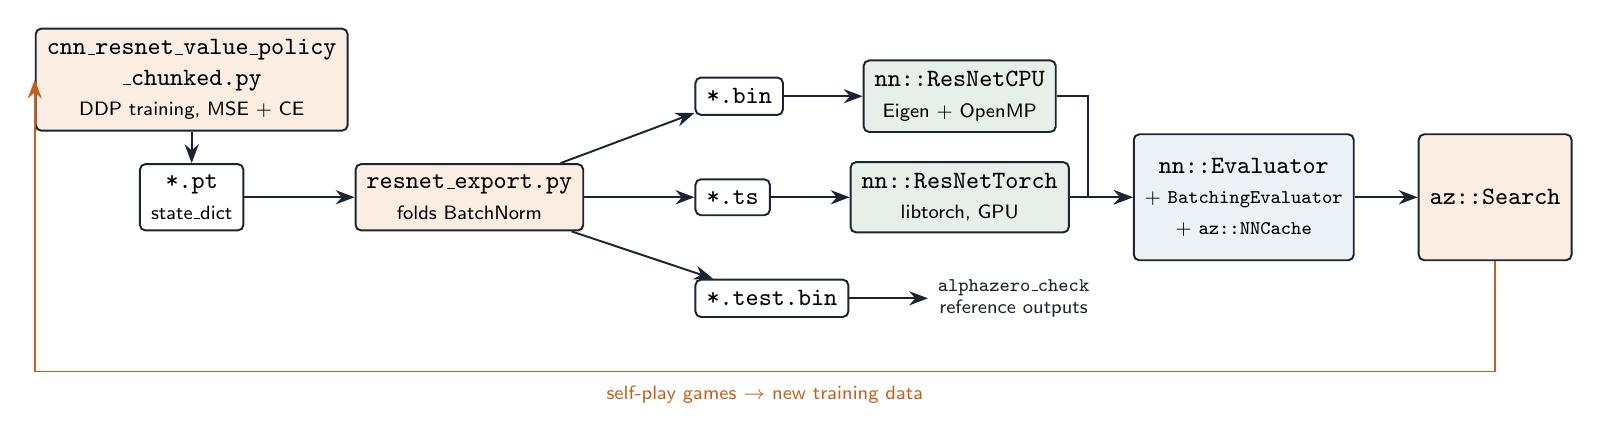
\begin{tikzpicture}[node distance=6mm]
  \node[boxa] (train) {\texttt{cnn\_resnet\_value\_policy}\\\texttt{\_chunked.py}\\\scriptsize DDP training, MSE + CE};
  \node[box,below=4mm of train,fill=white] (ckpt) {\texttt{*.pt}\\\scriptsize state\_dict};
  \node[boxa,right=14mm of ckpt] (exp) {\texttt{resnet\_export.py}\\\scriptsize folds BatchNorm};

  \node[box,above right=6mm and 14mm of exp,fill=white] (bin) {\texttt{*.bin}};
  \node[box,right=14mm of exp,fill=white] (ts) {\texttt{*.ts}};
  \node[box,below right=6mm and 14mm of exp,fill=white] (tb) {\texttt{*.test.bin}};

  \node[boxb,right=10mm of bin] (cpu) {\texttt{nn::ResNetCPU}\\\scriptsize Eigen + OpenMP};
  \node[boxb,right=10mm of ts] (torch) {\texttt{nn::ResNetTorch}\\\scriptsize libtorch, GPU};
  \node[plain,right=10mm of tb,font=\sffamily\scriptsize] (chk) {\texttt{alphazero\_check}\\reference outputs};

  \node[box,right=8mm of torch,minimum height=16mm] (ev) {\texttt{nn::Evaluator}\\\scriptsize + \texttt{BatchingEvaluator}\\\scriptsize + \texttt{az::NNCache}};
  \node[boxa,right=8mm of ev,minimum height=16mm] (mcts) {\texttt{az::Search}};

  \draw[ar] (train) -- (ckpt);
  \draw[ar] (ckpt) -- (exp);
  \draw[ar] (exp) -- (bin); \draw[ar] (exp) -- (ts); \draw[ar] (exp) -- (tb);
  \draw[ar] (bin) -- (cpu); \draw[ar] (ts) -- (torch); \draw[ar] (tb) -- (chk);
  \draw[ar] (cpu.east) -- ++(4mm,0) |- (ev.west);
  \draw[ar] (torch) -- (ev);
  \draw[ar] (ev) -- (mcts);
  \draw[ar,draw=accent2] (mcts.south) -- ++(0,-14mm) -| node[tiny,pos=.25,below,text=accent2,yshift=-.5mm]{self-play games $\to$ new training data} (train.west);
\end{tikzpicture}
\end{document}
